\section{Motivating Scenarios}
\label{s:deploy}
%\radhika{need a better title?}
\begin{figure*}
    \centering
    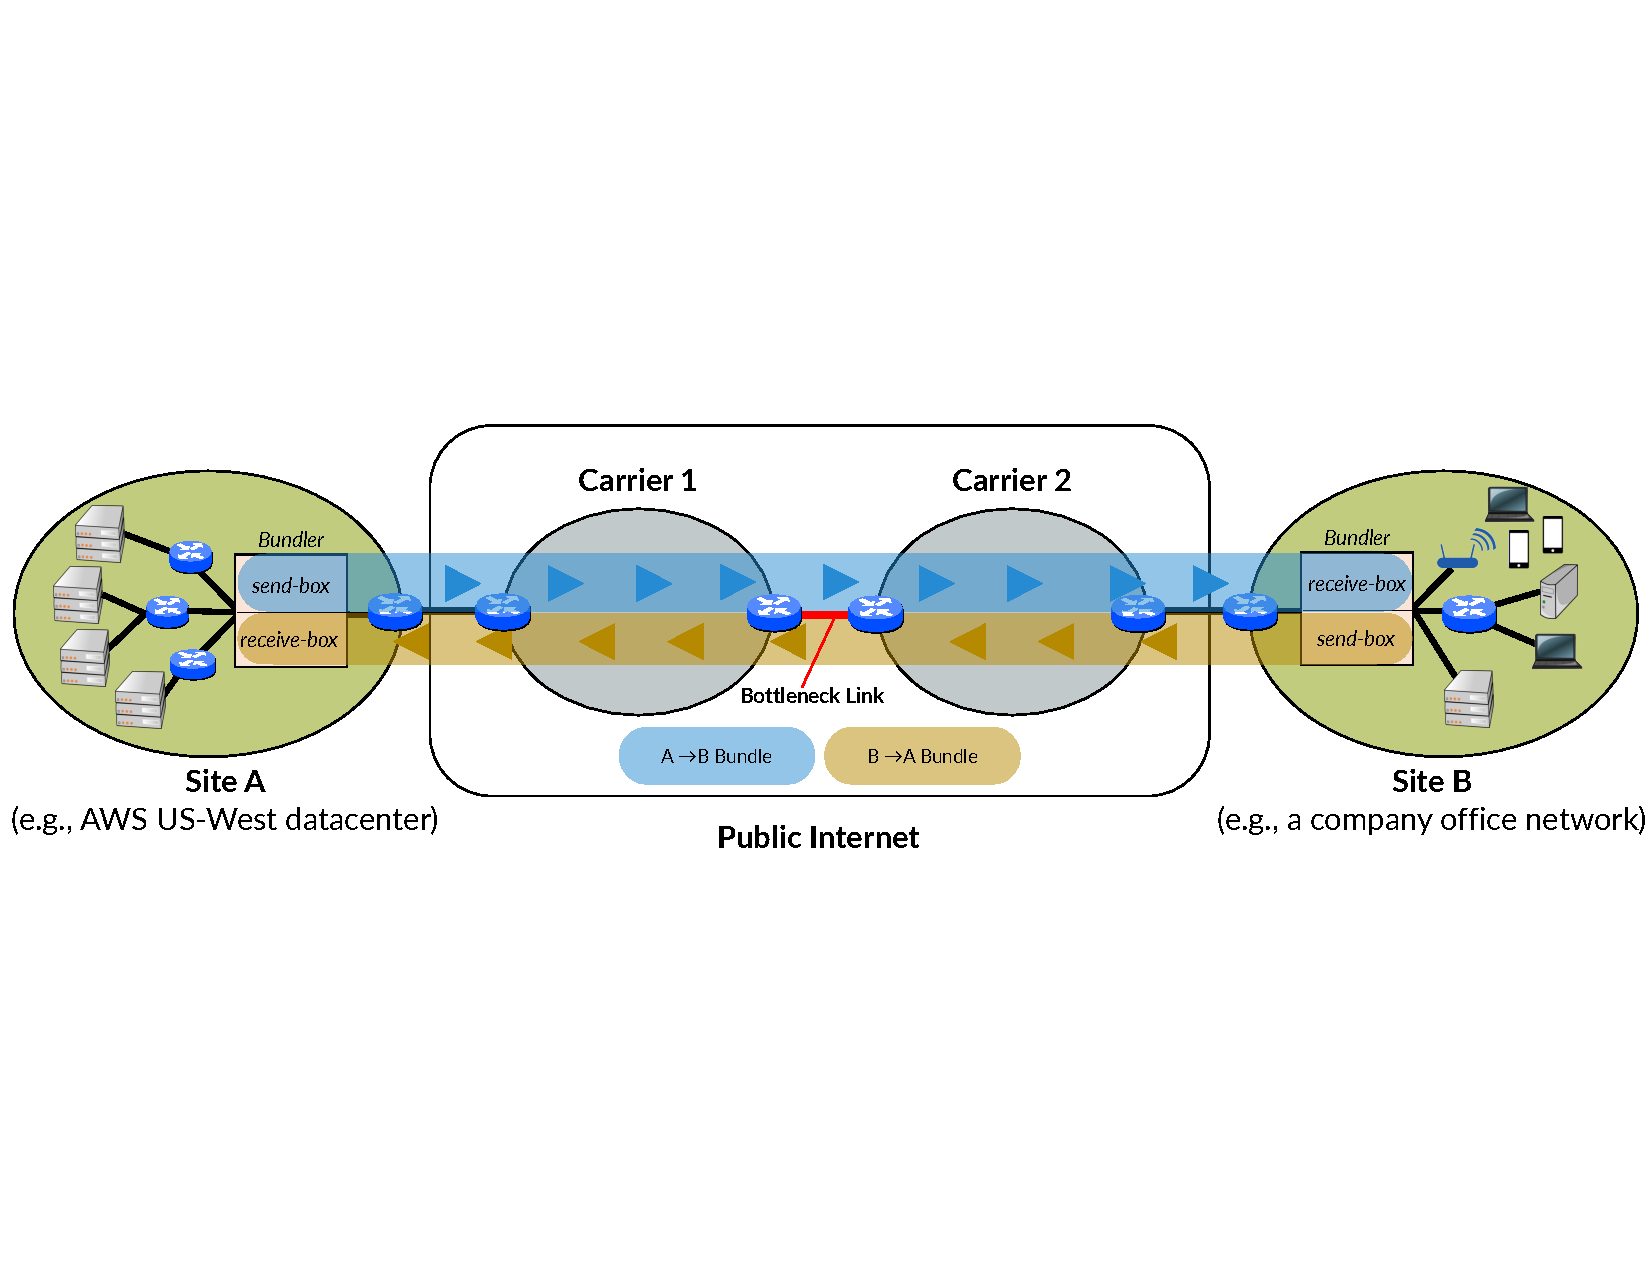
\includegraphics[width=\textwidth]{img/deployment-arch.pdf}
    \caption{Simplified respresentation of \name's deployment. 
    The \inbox sits at the sending domain's egress and \outbox sits at the receiving domain's ingress. All traffic  gets bundled together for scheduling. Bottleneck exists between the \inbox and the \outbox.
    }\label{fig:deploy:arch}
\end{figure*}

\radhika{outline:/*}

\name provides benefits over status quo, when the following conditions are met:

\Para{Opportunities for bundling traffic}
\begin{itemize}
    \item Cite venkat's hotnets and Labovitz paper (any other citations?)
\end{itemize}

\Para{Bottleneck in the middle of the network}
Can arise due to following:

\paragraphi{When carriers do rate limiting}
Find citations
\begin{itemize}
    \item can result in self-inflicted bottlenecks (any citations to show how common this is?).
    \item best case for bundler.
\end{itemize}

\paragraphi{Congestion from other traffic}
\begin{itemize}
    \item short-lived (up to a few MB) cross traffic: we still get benefits.
    \item other bundled traffic: we still get benefits.
    \item long-lived persistent connections: fall back to status quo.
\end{itemize}
\radhika{Also say something about placement of \inbox \outbox pairs.}

\Para{Bottleneck is shared by the bundled traffic}

\radhika{*/}